% ****** Start of file apssamp.tex ******
%
%   This file is part of the APS files in the REVTeX 4 distribution.
%   Version 4.0 of REVTeX, August 2001
%
%   Copyright (c) 2001 The American Physical Society.
%
%   See the REVTeX 4 README file for restrictions and more information.
%
% TeX'ing this file requires that you have AMS-LaTeX 2.0 installed
% as well as the rest of the prerequisites for REVTeX 4.0
%
% See the REVTeX 4 README file
% It also requires running BibTeX. The commands are as follows:
%
%  1)  latex apssamp.tex
%  2)  bibtex apssamp
%  3)  latex apssamp.tex
%  4)  latex apssamp.tex
%
\documentclass[prb,aps,twocolumn,preprintnumbers,amsmath,amssymb]{revtex4}
%\documentclass[preprint,showpacs,preprintnumbers,amsmath,amssymb]{revtex4}

% Some other (several out of many) possibilities
%\documentclass[preprint,aps]{revtex4}
%\documentclass[preprint,aps,draft]{revtex4}
%\documentclass[prb,twocolumn,showpacs,preprintnumbers,amsmath,amssymb]{revtex4}% Physical Review B

\usepackage{graphicx}% Include figure files
\usepackage{dcolumn}% Align table columns on decimal point
\usepackage{bm}% bold math
\usepackage[utf8]{inputenc}
\newcommand*{\Scale}[2][4]{\scalebox{#1}{$#2$}}%
%\nofiles

\begin{document}

\title{Carga específica del electrón - $e/m$}% Force line breaks with \\

\author{Alejandro Hernández A.}%
 \email{a.hernandez105@uniandes.edu.co}
\author{Daniel Sánchez M.}%
 \email{d.sanches462@uniandes.edu.co}
\affiliation{%
Departamento de Física\\ Universidad de los Andes, Bogotá, Colombia.\\
}%
\date{20 de agosto de 2015\\}% It is always \today, today,
             %  but any date may be explicitly specified

\begin{abstract}
Este informe presenta los datos obtenidos al medir la diferencia de potencial y la corriente con los cuales se curvaba un haz de electrones en trayectorias circulares de radios particulares. Conociendo las corrientes aplicadas sobre los anillos laterales de una bobina de Helmholtz y usando las ley de Biot-Savart y la fuerza de Lorentz, se obtuvo un valor experimental para al carga específica del electrón, a saber, $\left( e/m_{e} \right) = (1.550 \pm 0.050) \cdot 10^{11} \frac{C}{kg}$ con un error porcentual de  $E\% = 11.831\%$.
\\

%\smallskip
\noindent \textbf{Conceptos clave:} Bobina de Helmholtz, ley de Biot-Savart, fuerza de Lorentz.
\end{abstract}
                             
\maketitle

\section{\label{sec:level1}Introducción.}

La carga específica de una partícula con carga $q$ y masa $m$ se define como la razónentre estas cantidades $q/m$. Para el caso particular del electrón, la razón carga-masa fue medida por primera vez por J.J. Thompson en el año de 1897. Al obtener un valor negaivo, confirmó la predicción de Lorentz acerca de la existencia de una partícula subatómica de carga menor que cero. Este descubrimiento produjo un cambio en el modelo atómico de la época, de acuerdo al cual el átomo era una esfera indivisible de carga neutra. De esta forma, el mismo Thompson propuso un nuevo modelo que sugería una distribución homogénea de electrones dentro de una esfera sólida. A pesar de que este modelo no resultó ser satisfactorio, su importancia yace en considerar al átomo como un conglomerado de diversos elementos con carga elétrica y no como un todo indivisible.\\

Si un electrón de masa $m_{e}$ y carga $e$ es acelerado por una diferencia de potencial $V$, por conservación de la energía se tiene:

\begin{equation}
\label{cons. ener.}
eV = \frac{1}{2} m_{e} v^2
\end{equation}

\noindent
donde $v$ es la velocidad del electrón.\\

En presencia de un campo magnético $\vec{B}$, la fuerza de Lorentz que actúa sobre un electrón con velocidad $\vec{v}$ es: 

\begin{equation}
\vec{F} = e\cdot\vec{v}\times\vec{B}
\end{equation}

En general, el electrón describe un trayectoria en forma de espiral alrededor de la dirección del campo, y en el caso particular en que $\vec{v}$ y $\vec{B}$ sean perpendiculares, la trayectoria es circular. En este último caso, la fuerza de Lorentz es una fuerza centrífuga $F = \frac{m_{e}v^2}{r}$, con lo cual se tiene que 

\begin{equation}
\label{velocidad}
v = \frac{e}{m_{e}} \cdot Br
\end{equation}

\noindent
donde $r$ es el radio de la trayectoria descrita por el electrón.\\
\indent
Reemplazando \eqref{velocidad} en \eqref{cons. ener.} se obtiene:

\begin{equation}
\label{carga-masa}
\frac{e}{m_{e}} = \frac{2V}{(Br)^2}
\end{equation}

Ahora bien, para determinar $B$ es preciso usar la ley de Biot-Savart. El campo magnético $B_{z}$ sobre e eje z de un arreglo simétrico de dos embobinados de radio $R$, separados una distancia $a$, por los cuales circula una corriente $I$ es:

\begin{equation*}
\Scale[0.98]{
B_{z} = \frac{\mu_{0}IR^2}{2}\left[ \left( R^2 + \left(z - \frac{a}{2}\right)^2 \right)^{-3/2} + \left( R^2 + \left(z + \frac{a}{2}\right)^2 \right)^{-3/2} \right]
}
\end{equation*}

\noindent
donde $\mu_{0} = 1.257\cdot10^{-6} \frac{Vs}{Am}$ es la permeabilidad magnética del vacío.\\

Para una bobina de Hemmholtz con n vueltas en cada emobinado, $a = R$ y $z = 0$ se tiene que 

\begin{equation}
\label{campo helm.}
B = \left(\frac{4}{5}\right)^{3/2} \mu_{0}\cdot n\cdot \frac{I}{R}
\end{equation}

\section{Montaje experimental}

Con el fin de medir la carga específica del electrón, se utilizó un \textit{narrow beam tube} para acelerar un haz de electrones que era curvado en una trayectoria circular debido a la presencia de un campo magnético generado por una bobina de Helmholtz.\\

Para la alimentación del \textit{narrow beam tube} se usó una fuente de voltaje de capacidad máxima $300V$, que permitía fuertes variaciones en la energía cinética del haz de electrones. En contraste con lo anterior, para la bobina de Helmholtz se utilizó una fuente de capacidad máxima $18V$, que generaba corrientes entre $2A$ y $4A$, lo suficiente grandes para que el campo magnético afecte visiblemente la trayectoria del haz.\\

El montaje experimental usado durante la práctica se muestra en la figura \ref{fig:montaje}.\\\\\\

\begin{widetext}
	
	\begin{figure}[h!]
		\centering
		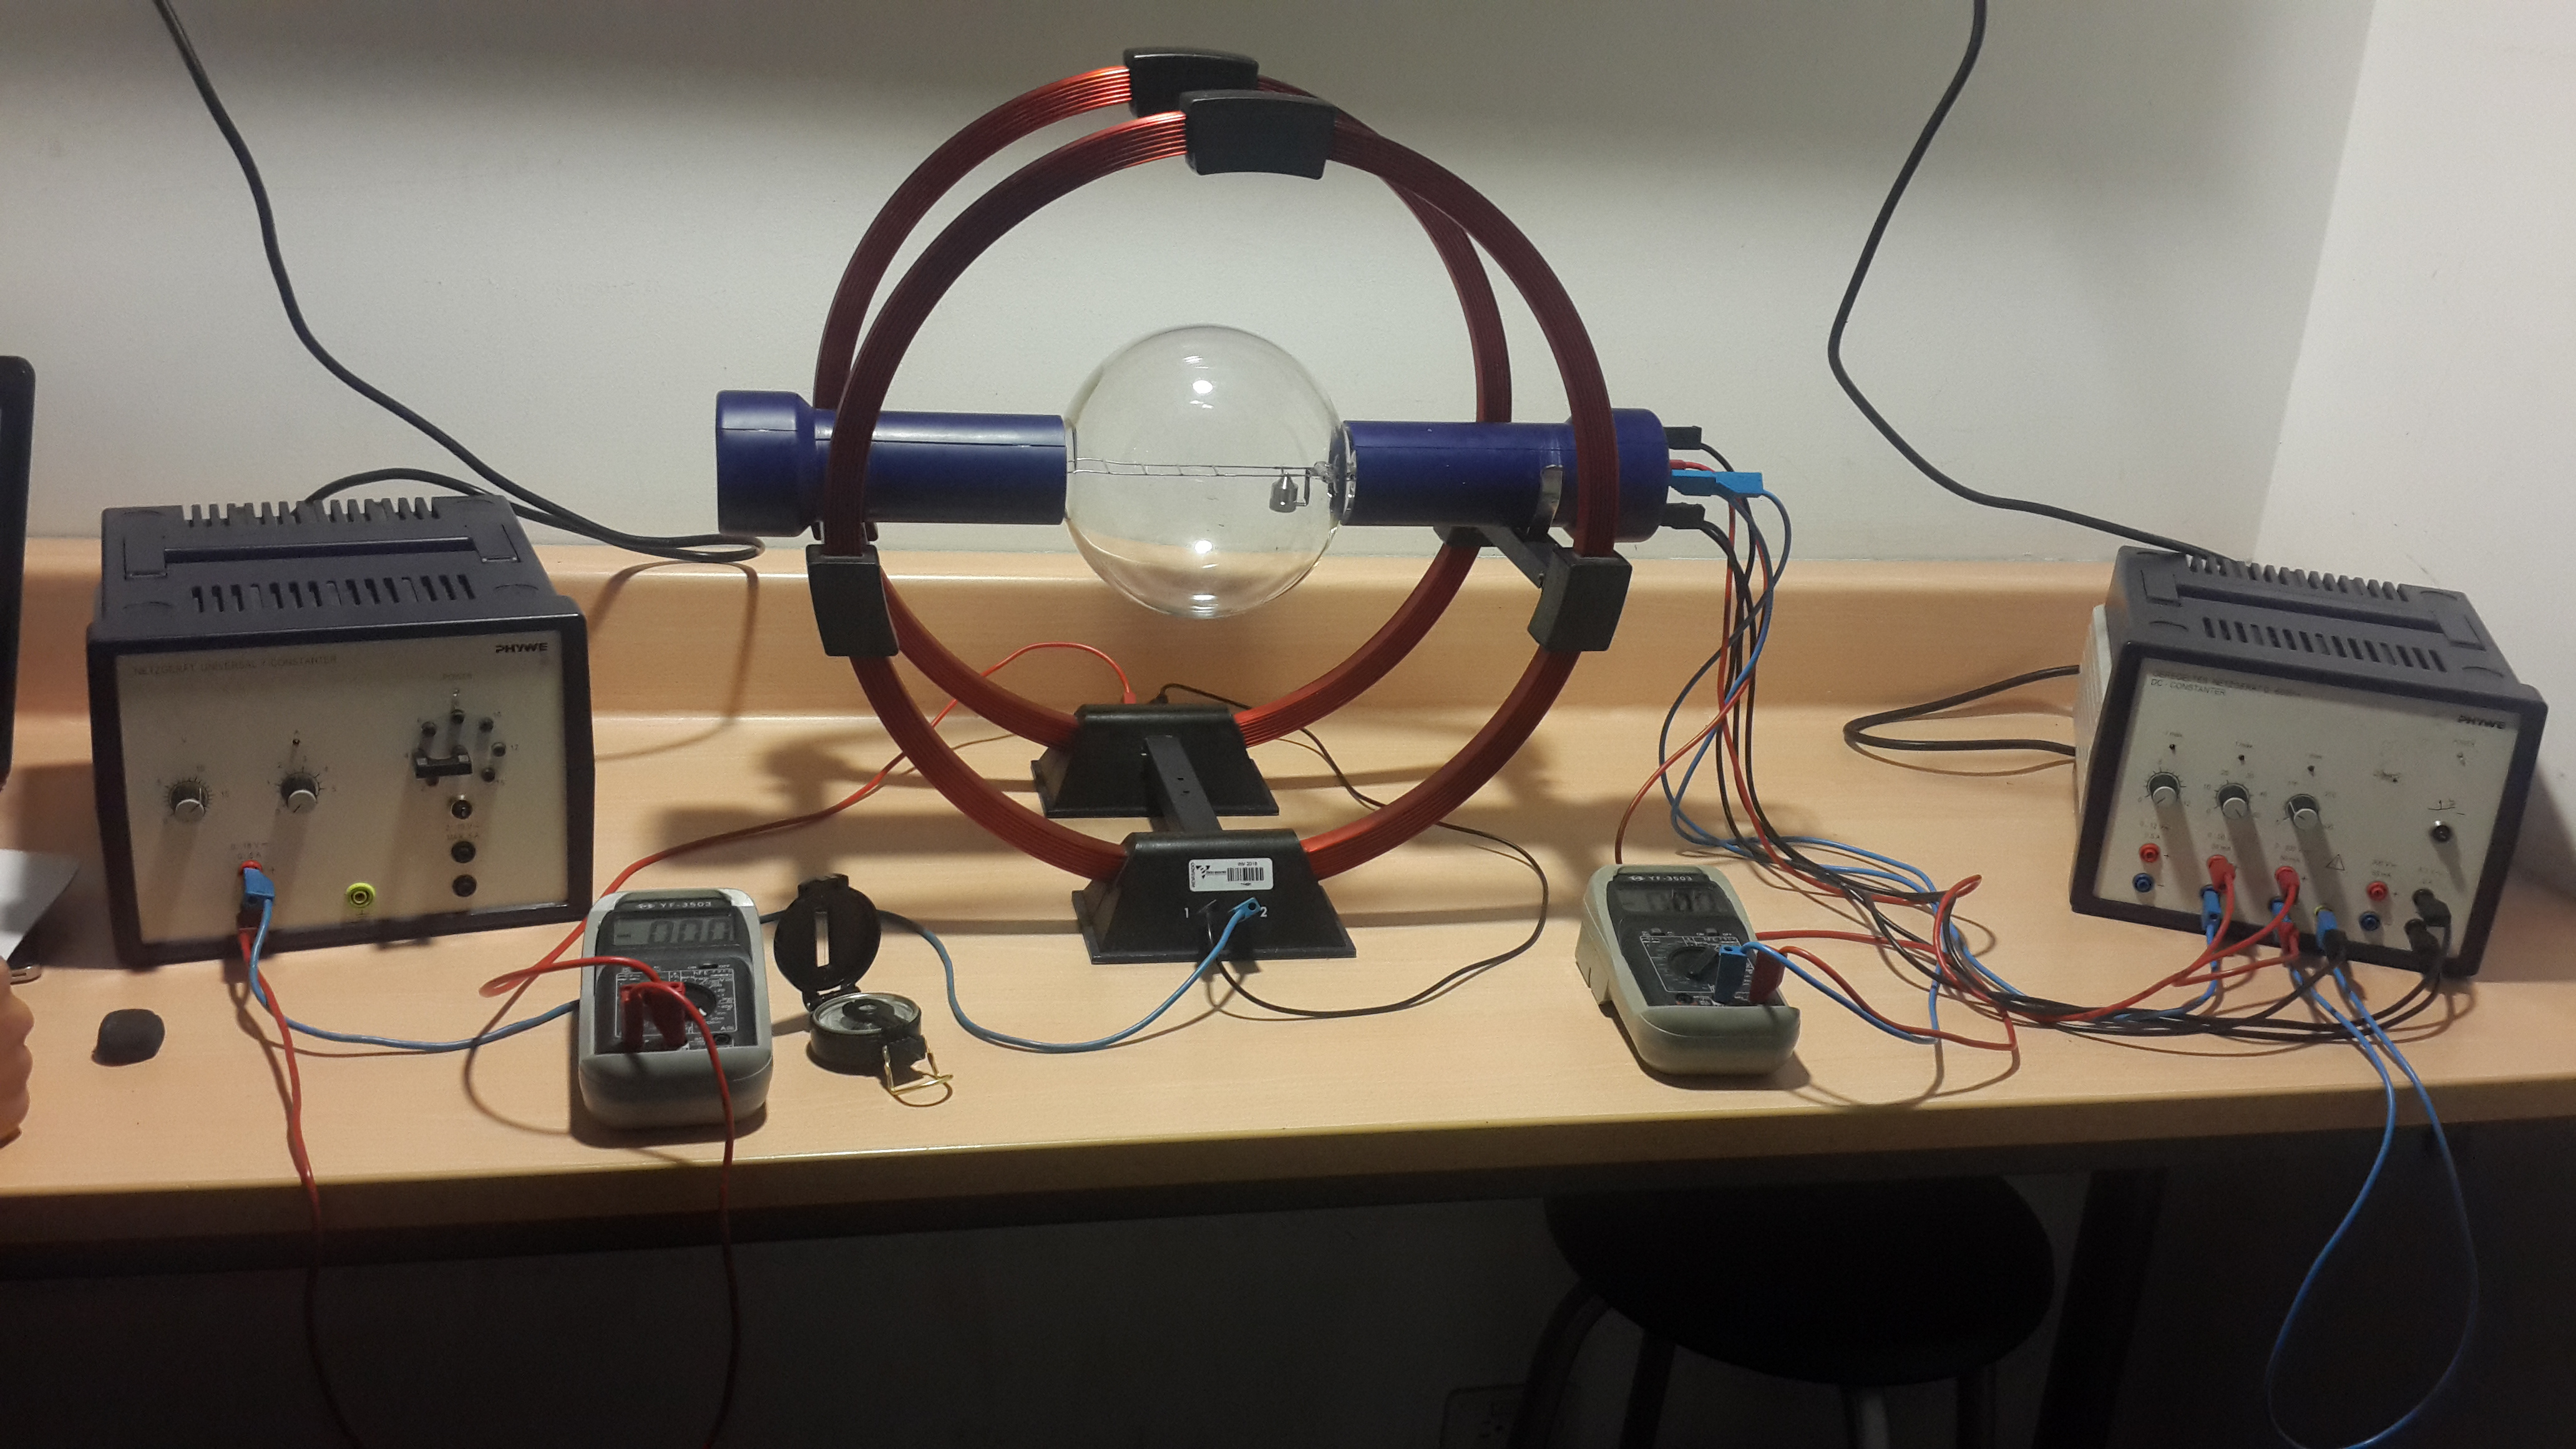
\includegraphics[width=0.7\textwidth]{carga-masa}
		\caption{Montaje experimental}
		\label{fig:montaje}
	\end{figure}
	
\end{widetext}

\begin{figure}[h!]
	\centering
	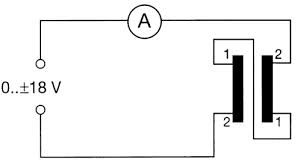
\includegraphics[width=0.4\textwidth,height=0.1\textheight]{helmholtz-coils}
	\caption{Diagrama de conexión para la bobina de Helmholtz.}
	\label{fig:coils}
\end{figure}

\begin{figure}[h!]
	\centering
	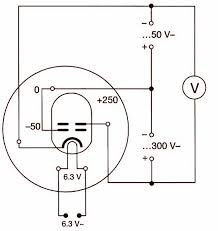
\includegraphics[width=0.5\textwidth,height=0.25\textheight]{narrow-beam-tube}
	\caption{Diagrama de conexión para el \textit{narrow beam tube}.}
	\label{fig:tube}
\end{figure}

Por otra parte, en las figuras \ref{fig:coils} y \ref{fig:tube} se muestran los circuitos utilizados para conectar la bobina de Helmholtz y el \textit{narrow beam tube} respectivamente. Cabe notar que en el montaje observado en la figura \ref{fig:montaje}, el amperímetro es el encargado de medir la corriente que pasa a través de la bobina de Helmholtz y, de acuerdo a \eqref{campo helm.}, el dispositivo que permite conocer el campo magnético que curva al haz; por su parte, el voltímetro permite conocer la diferencia de potencial que acelera el haz de electrones.\\

Una vez hechas las conexiones, basta con encender ambas fuentes y asignar valores específicos de voltaje del \textit{narrow beam tube} y de corriente de las bobinas, para observar un haz de color cian tenue que se contrae formando una circunferencia debido al campo magnético, cuyo radio se puede ajustar para que tome valores fijos de $2,\ 3,\ 4$ y $5\ cm$, distancias que se encuentran marcadas en el \textit{narrow beam tube}, de manera que cuando el haz pasa a través de ellas se corta en dos o reduce su intensidad bruscamente, lo cual permite una medición confiable de dichos radios.\\\\\\\\\\\\



\section{Resultados y análisis}

Los resultados de las mediciones de corriente y voltaje se muestran en la Tabla \ref{Tabla 1}.\\

\begin{table}[h!]
	\caption{\label{Tabla 1}Voltaje y corriente para.}
	\begin{ruledtabular}
		\begin{tabular}{ccccc}
			\multicolumn{1}{c}{$V \pm 1V$} & \multicolumn{4}{c}{$A \pm 0.01A$ } \\
			\hline
			Voltaje &$I_{2\ cm}$&$I_{3\ cm}$&$I_{4\ cm}$&$I_{5\ cm}$\\
			\hline
			110 & 2.60 & 1.44 & 1.11 & 0.85 \\
			120 & 2.73 & 1.73 & 1.21 & 0.92\\
			130 & 2.79 & 1.17 & 1.30 & 0.96\\
			140 & 2.83 & 1.86 & 1.35 & 1.02\\
			150 & 2.96 & 1.87 & 1.39 & 1.08\\
			160 & 3.06 & 1.99 & 1.41 & 1.13\\
			170 & 3.17 & 2.03 & 1.47 & 1.17\\
			180 & 3.28 & 2.09 & 1.53 & 1.22\\
			190 & 3.38 & 2.15 & 1.58 & 1.25\\
			200 & 3.46 & 2.21 & 1.63 & 1.30\\
			210 & 3.60 & 2.28 & 1.68 & 1.33\\
			220 & 3.68 & 2.33 & 1.72 & 1.36\\
			230 & 3.73 & 2.40 & 1.77 & 1.40\\
			240 & 3.79 & 2.46 & 1.81 & 1.43\\
			250 & 3.90 & 2.50 & 1.84 & 1.46\\
			260 & 3.98 & 2.56 & 1.89 & 1.49\\
			270 & 4.05 & 2.62 & 1.93 & 1.53\\
		\end{tabular}
	\end{ruledtabular}
\end{table}

Con el fin de analizar los datos, es conveniente ver \eqref{carga-masa} de la siguiente manera:

\begin{equation}
V = \frac{e}{m_{e}}\cdot\frac{(Br)^2}{2} 
\label{lineal}
\end{equation}

Identificando $\frac{(Br)^2}{2} \rightarrow x$ y $V \rightarrow y$, se puede ver en la figura \ref{fig:lineal} que los datos efectivamente satisfacen la relación dada por \eqref{lineal}, razón por la cual se justifica hacer una regresión lineal de los datos.\\

\begin{figure}[h!]
	\centering
	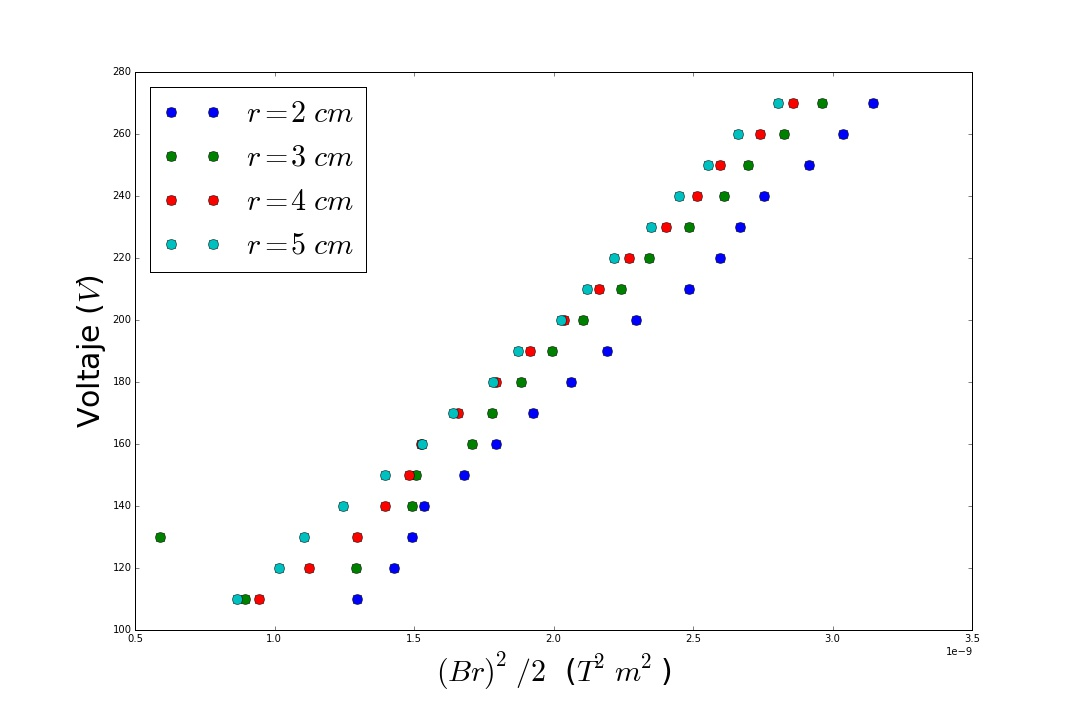
\includegraphics[width=0.55\textwidth]{carga-masa-reg}
	\caption{Voltaje en función $\frac{(B(I)r)^2}{2}$ para diversos los diversos radios.}
	\label{fig:lineal}
\end{figure}

Con lo anterior, se obtiene el siguiente valor para la carga específica del electrón:

\begin{equation}
\left( \frac{e}{m_{e}} \right)_{exp} = (1.550 \pm 0.050) \cdot 10^{11} \frac{C}{kg} 
\end{equation}

Y al comparar con el valor teórico\footnote{Valor obtenido de https://en.wikipedia.org/wiki/Mass-to-charge\_ratio} de dicha constante, $\left( \frac{e}{m_{e}} \right)_{teo} = (1.758 \cdot 10^{11}  \pm 39)  \frac{C}{kg}$, el cálculo del error porcentual arroja un resultado de $E\% = 11.831\%$.\\

Es preciso mencionar que hubo múltiples factores que generaron dicho error, entre ellos destacan los siguientes:

\begin{itemize}
	\item Se observó que los datos de corriente y voltaje que generaban una determinada curvatura del haz de electrones variaban mucho estando cerca de los radios marcados en el \textit{narrow beam tube}, y dado a que se requería que el haz pasara justo por encima de las marcas, consideramos que esta difucltad fue la que causó el error sistemático más significativo del experimento.
	
	\item Además de lo mencionado anteriormente, fue difícil ajustar el \textit{narrow beam tube} de tal forma que solo se observara un círculo y no una espiral como trayectoria del haz de electrones, complicando de esta manera la realización de medidas completamente satisfactorias.
\end{itemize}
	
Continuando con los errores que ocurrieron durante e laboratorio, es preciso hablar de la forma en la que se calculó el campo magnético inducido. Para poder obtener una expresión para el campo, se asumió que la órbita del haz de eletrones estaba ubicada justamente en el centro de las espiras y, por tanto, experimentaba un campo magnético dado por \eqref{campo helm.} sobre todos los puntos de la trayectoria del haz. Sin embargo, la órbita no coincidía exactamente con el centro del círculo y por ende, el campo magnético estaba dado por la expresión dada para $B_{z}$ con $z \neq 0$. En adición a lo anterior, dado que $\frac{dB_{z}}{dz} \neq 0$ para $z \neq 0$, esto indica que si bien el campo varía poco en la vecidad de $z = 0$, dicho campo no es uniforme y sería preciso considerar sus variaciones en en análisis de datos con el fin de obtener medidas más confiables.\\  


Análogamente, para la simplificación del cálculo de la fuerza de Lorentz se asumió que el campo cruzaba el plano vertical definido por el haz a un ángulo exacto $ \pi /2 $. Claramente, el hecho de que no se tengan en cuenta pequeñas variaciones de este ángulo pudo producir desviaciones que, aunque minúsculas, vale la pena mencionar. \\

También hay que tener en cuenta que , en las mediciones realizadas, se está despreciando completamente el campo magnético de la Tierra, el cual oscila entre ($25-75 \mu T$), apenas un orden de magnitud más pequeño que el de los campos manéticos generados por las bobinas de Helmholtz para los radios más grandes ($4$ y $5$ cm) los cuales se encuentran entre los $500$ y los $1000 \mu T$ para valores bajos de potencial. Todo esto fortalece aún más la idea de que la estimación realizada más confiable es la que corresponde al anillo de radio $2cm$ el cual  es el menos distorsionado por el campo magnético terrestre debido a que para formar un anillo de este tamaño se necesita un campo magnético bastante fuerte ( Entre $1$ y $2 mT$). Esto nos muestra que si el experimento se realiza con el haz de electrones paralelo al campo magnético terrestre se podría obtener una medición más confiable de los datos obtenidos, especialmente de aquellos cuyo radio es más grande. \\

Por último , vale la pena destacar la gran magnitud que tiene esta constante, especialmente comparada con la carga especíca del proton cuyo valor es aproximadamente $9.578 \cdot 10^7 C/kg$, cuatro ordenes de magnitud menor a la carga específica del electrón, hecho que fue determinante para establecer la existencia de dos tipos de partículas cargadas dentro del átomo, una de ellas de masa mil veces menor que la otra.\\


\section{Conclusiones}

\begin{itemize}
	
	\item El valor experimental obtenido para la carga específica del electrón $\left( \frac{e}{m_{e}} \right)_{exp} = (1.631 \pm 0.041) \cdot 10^{11} \frac{C}{kg}$ no es muy exacto dado a que el error porcentual de la medida fue de $E\% = 10.104\%$.
		
	\item La observación realizada de esta carga específica permite validar experimentalmente la idea acerca de la divisibilidad del átomo y su composición de partículas de carga tanto positiva como negativa, cuyas cargas se compensan perfectamente para formar un átomo neutro.
	
	\item Si bien se obtuvieron buenos resultados, es importante resaltar que tanto la intensidad de las trayectorias observadas, como el grosor de las mismas y la dificultad para ver círculos y no espirales, da pie para pensar acerca de la realización de medidas con instrumentos de mayor resolución con el fin de obtener mediciones más exactas de la razón carga masa.
	
\end{itemize}

\begin{thebibliography}{99}
\bibitem{eisberg} R. Eisberg, {\it Quantum Physics of Atoms, Molecules, Solids, Nuclei and Particles}{John Wiley \& Sons, USA, 1985}.\\

\bibitem{Tipler} Tipler, Paul A., \textit{Physics for scientists and engineers}. W.H. Freeman, 4 Edici\' on, 1999.\\
\bibitem{Taylor} Taylor, J.R., \textit{An Introduction to Error Analysis}. University Science Books, Sausalito, California. 2nd edition, 1982.\\
\bibitem{Guia} Phywe. Specific Charge of the Electron -e/m. 5.1.02-00\\
\end{thebibliography}

\end{document}
%
% ****** End of file apssamp.tex ******
